\begin{enumerate}[label=\thesection.\arabic*,ref=\thesection.\theenumi]
\item Find the sum of the vectors $\vec{a}=\hat{i}-2\hat{j}+\hat{k}$, $\vec{b}=-2\hat{i}+4\hat{j}+5\hat{k}$ and $\vec{c}=\hat{i}-6\hat{j}-7\hat{k}$.
\item 

	In triangle ABC (Fig 10.18), which of the following is not true:
 \begin{enumerate}
         \item $\overrightarrow{AB}+\overrightarrow{BC}+\overrightarrow{CA}$=$\vec{0}$
         \item $\overrightarrow{AB}+\overrightarrow{BC}-\overrightarrow{CA}$=$\vec{0}$
         \item $\overrightarrow{AB}+\overrightarrow{BC}-\overrightarrow{CA}$=$\vec{0}$
         \item $\overrightarrow{AB}-\overrightarrow{BC}+\overrightarrow{CA}$=$\vec{0}$
\end{enumerate}
\begin{figure}[!ht]
\centering
\includegraphics[width = \columnwidth]{./chapters/12/10/2/18/figs/triangle.png}
\caption{}
	\label{fig:chapters/12/10/2/18/}
\end{figure}
\solution
		\iffalse
\documentclass[journal,12pt,twocolumn]{IEEEtran}
\usepackage{romannum}
\usepackage{float}
\usepackage{setspace}
\usepackage{gensymb}
\singlespacing
\usepackage[cmex10]{amsmath}
\usepackage{amsthm}
\usepackage{mathrsfs}
\usepackage{txfonts}
\usepackage{stfloats}
\usepackage{bm}
\usepackage{cite}
\usepackage{cases}
\usepackage{subfig}
\usepackage{longtable}
\usepackage{multirow}
\usepackage{enumitem}
\usepackage{mathtools}
\usepackage{steinmetz}
\usepackage{tikz}
\usepackage{circuitikz}
\usepackage{verbatim}
\usepackage{tfrupee}
\usepackage[breaklinks=true]{hyperref}
\usepackage{tkz-euclide}
\usetikzlibrary{calc,math}
\usepackage{listings}
    \usepackage{color}                                            %%
    \usepackage{array}                                            %%
    \usepackage{longtable}                                        %%
    \usepackage{calc}                                             %%
    \usepackage{multirow}                                         %%
    \usepackage{hhline}                                           %%
    \usepackage{ifthen}                                           %%
  %optionally (for landscape tables embedded in another document): %%
    \usepackage{lscape}     
\usepackage{multicol}
\usepackage{chngcntr}
\DeclareMathOperator*{\Res}{Res}
\renewcommand\thesection{\arabic{section}}
\renewcommand\thesubsection{\thesection.\arabic{subsection}}
\renewcommand\thesubsubsection{\thesubsection.\arabic{subsubsection}}

\renewcommand\thesectiondis{\arabic{section}}
\renewcommand\thesubsectiondis{\thesectiondis.\arabic{subsection}}
\renewcommand\thesubsubsectiondis{\thesubsectiondis.\arabic{subsubsection}}

% correct bad hyphenation here
\hyphenation{op-tical net-works semi-conduc-tor}
\def\inputGnumericTable{}                                 %%

\lstset{
frame=single, 
breaklines=true,
columns=fullflexible
}

\begin{document}


\newtheorem{theorem}{Theorem}[section]
\newtheorem{problem}{Problem}
\newtheorem{proposition}{Proposition}[section]
\newtheorem{lemma}{Lemma}[section]
\newtheorem{corollary}[theorem]{Corollary}
\newtheorem{example}{Example}[section]
\newtheorem{definition}[problem]{Definition}
\newcommand{\BEQA}{\begin{eqnarray}}
\newcommand{\EEQA}{\end{eqnarray}}
\newcommand{\define}{\stackrel{\triangle}{=}}

\bibliographystyle{IEEEtran}
\providecommand{\mbf}{\mathbf}
\providecommand{\pr}[1]{\ensuremath{\Pr\left(#1\right)}}
\providecommand{\qfunc}[1]{\ensuremath{Q\left(#1\right)}}
\providecommand{\sbrak}[1]{\ensuremath{{}\left[#1\right]}}
\providecommand{\lsbrak}[1]{\ensuremath{{}\left[#1\right.}}
\providecommand{\rsbrak}[1]{\ensuremath{{}\left.#1\right]}}
\providecommand{\brak}[1]{\ensuremath{\left(#1\right)}}
\providecommand{\lbrak}[1]{\ensuremath{\left(#1\right.}}
\providecommand{\rbrak}[1]{\ensuremath{\left.#1\right)}}
\providecommand{\cbrak}[1]{\ensuremath{\left\{#1\right\}}}
\providecommand{\lcbrak}[1]{\ensuremath{\left\{#1\right.}}
\providecommand{\rcbrak}[1]{\ensuremath{\left.#1\right\}}}
\theoremstyle{remark}
\newtheorem{rem}{Remark}
\newcommand{\sgn}{\mathop{\mathrm{sgn}}}
\providecommand{\abs}[1]{\left\vert#1\right\vert}
\providecommand{\res}[1]{\Res\displaylimits_{#1}} 
\providecommand{\norm}[1]{\left\lVert#1\right\rVert}
\providecommand{\mtx}[1]{\mathbf{#1}}
\providecommand{\mean}[1]{E\left[ #1 \right]}
\providecommand{\fourier}{\overset{\mathcal{F}}{ \rightleftharpoons}}
\providecommand{\system}{\overset{\mathcal{H}}{ \longleftrightarrow}}
\newcommand{\solution}{\noindent \textbf{Solution: }}
\newcommand{\cosec}{\,\text{cosec}\,}
\providecommand{\dec}[2]{\ensuremath{\overset{#1}{\underset{#2}{\gtrless}}}}
\newcommand{\myvec}[1]{\ensuremath{\begin{pmatrix}#1\end{pmatrix}}}
\newcommand{\mydet}[1]{\ensuremath{\begin{vmatrix}#1\end{vmatrix}}}
\numberwithin{equation}{subsection}
\makeatletter
\@addtoreset{figure}{problem}
\makeatother

\let\StandardTheFigure\thefigure
\let\vec\mathbf
\renewcommand{\thefigure}{\theproblem}



\def\putbox#1#2#3{\makebox[0in][l]{\makebox[#1][l]{}\raisebox{\baselineskip}[0in][0in]{\raisebox{#2}[0in][0in]{#3}}}}
     \def\rightbox#1{\makebox[0in][r]{#1}}
     \def\centbox#1{\makebox[0in]{#1}}
     \def\topbox#1{\raisebox{-\baselineskip}[0in][0in]{#1}}
     \def\midbox#1{\raisebox{-0.5\baselineskip}[0in][0in]{#1}}

\vspace{3cm}


\title{Assignment 1}
\author{Jaswanth Chowdary Madala}





% make the title area
\maketitle

\newpage

%\tableofcontents

\bigskip

\renewcommand{\thefigure}{\theenumi}
\renewcommand{\thetable}{\theenumi}

\begin{enumerate}
\item In the following figure for the triangle ABC, which of the following is not true:

(A) $\overrightarrow{AB}+\overrightarrow{BC}+\overrightarrow{CA} = \overrightarrow{0}$

(B) $\overrightarrow{AB}+\overrightarrow{BC}-\overrightarrow{AC} = \overrightarrow{0}$

(C) $\overrightarrow{AB}+\overrightarrow{BC}+\overrightarrow{AC} = \overrightarrow{0}$

(D) $\overrightarrow{AB}-\overrightarrow{CB}+\overrightarrow{CA} = \overrightarrow{0}$

\textbf{Solution:}
\fi
		We know that,
\begin{align}
\overrightarrow{AB} = \vec{B} - \vec{A}\\
\overrightarrow{BC} = \vec{C} - \vec{B}\\
\overrightarrow{CA} = \vec{A} - \vec{C}
\end{align}
By usinig this we verify each of the given option

\begin{enumerate}
\item 
\begin{align}
\overrightarrow{AB}+\overrightarrow{BC}+\overrightarrow{CA} &=
\vec{B}-\vec{A} + \vec{C} - \vec{B} + \vec{A} - \vec{C}\\
 &= 0
\end{align}
Option A is correct.

\item
\begin{align}
\overrightarrow{AB}+\overrightarrow{BC}-\overrightarrow{AC} &=
\vec{B}-\vec{A} + \vec{C} - \vec{B} - (\vec{C} - \vec{A})\\
 &= 0
\end{align}
Option B is correct.

\item 
\begin{align}
\overrightarrow{AB}+\overrightarrow{BC}+\overrightarrow{AC} &=
\vec{B}-\vec{A} + \vec{C} - \vec{B} + \vec{C} - \vec{A}\\
 &= 2(\vec{C}-\vec{A})
\end{align}
Option C is incorrect.

\item
\begin{align}
\overrightarrow{AB}-\overrightarrow{CB}+\overrightarrow{CA} &=
\vec{B}-\vec{A} - (\vec{B} - \vec{C}) + \vec{A} - \vec{C}\\
 &= 0
\end{align}
Option D is correct.
\end{enumerate}
Verification: Let us take an example to verify 
\begin{align}
\vec{A} = \myvec{1\\1}, 
\vec{B} = \myvec{3\\1},
\vec{C} = \myvec{6\\6} \\
\overrightarrow{AB} = \vec{B} - \vec{A} = \myvec{2\\0}, 
\overrightarrow{BC} = \vec{C} - \vec{B} = \myvec{3\\5},
\overrightarrow{CA} = \vec{A} - \vec{C} = \myvec{-5\\-5} 
\end{align}
Thus,
\begin{align}
\overrightarrow{AB}+\overrightarrow{BC}+\overrightarrow{CA} = \myvec{2+3+(-5) \\ 0+5+(-5)} = \myvec{0 \\0}
\end{align}
Similarly other options can be verified.



\item If $\vec{a}$ and $\vec{b}$ are two collinear vectors, then which of the following are incorrect:
\begin{enumerate}
    \item $\vec{b}=\lambda\vec{a},$
 for some scalar $\lambda$
    \item $\vec{a}=\pm\vec{b}$
    \item the respective components of $\vec{a}$ and $\vec{b}$ are not proportiona
    \item both the vectors $\vec{a}$ and $\vec{b}$ have same direction, but different magnitudes.
\end{enumerate}
	\item If a line makes angles $90\degree,135\degree,45\degree$ with x,y and z-axis respectivly. Find its direction cosines.
		\\
		\solution
				From \eqref{eq:dir-vec-3d},
the direction vector is
\begin{align}
\vec{A}=\myvec{\cos 90\degree\\ \cos 135\degree\\ \cos 45\degree}=\myvec{0\\-\frac{1}{\sqrt{2}}\\ \frac{1}{\sqrt{2}}}
\end{align}

\item A girl walks 4 km towards west, then she walks 3 km in a direction 30$^{\circ}$ east of north and stops. Determine the girl's displacement from her initial point of departure.\\
	\solution
		See  
\figref{fig:chapters/12/10/5/3Fig1}.
Let the initial position
be
\begin{align}
	\vec{A}=\myvec{0\\0}
\end{align}
After going west, the position becomes
\begin{align}
			\vec{B}=\myvec{-4\\0}
\end{align}
If the final position be $\vec{C}$, from the given information,
\begin{align}
	 \vec{C}-\vec{B}=3\myvec{\cos{60\degree}\\\sin{60\degree}}
	 \implies 
	\vec{C}  
=\myvec{\frac{-5}{2}\\[2pt] \frac{3\sqrt{3}}{2}}
\end{align}
which is the desired displacement. 
\begin{figure}[H] 
 \begin{center} 
 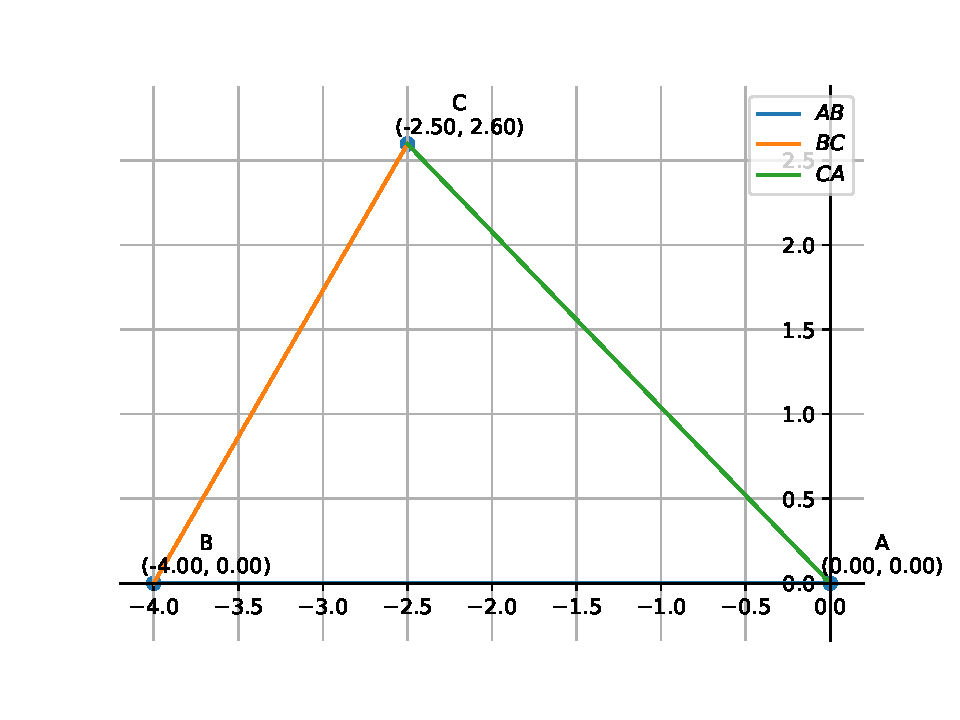
\includegraphics[width=0.75\columnwidth]{chapters/12/10/5/3/figs/fig.pdf} 
 \end{center} 
\caption{} 
\label{fig:chapters/12/10/5/3Fig1} 
\end{figure}

\item If $\vec{a}=\hat{i}+\hat{j}+\hat{k}$,$\vec{b}=2\hat{i}-\hat{j}+3\hat{k}$ and $\vec{c}=\hat{i}-2\hat{j}+\hat{k}$, find a unit vector parallel to the vector $2\vec{a}-\vec{b}+3\vec{c}$.\\
	\solution
		\begin{align}
2\vec{a}-\vec{b}+3\vec{c}=\myvec{3\\-3\\2}
\implies
\frac{2\vec{a}-\vec{b}+3\vec{c}}{\norm{2\vec{a}-\vec{b}+3\vec{c}}}
=\frac{1}{\sqrt{22}}\myvec{3\\-3\\2}
\end{align}


\item The two opposite vertices of a square are $(–1, 2)$  and $ (3, 2)$. Find the coordinates of the other two vertices.
\\
	\iffalse
\documentclass[12pt]{article}
\usepackage{graphicx}
\usepackage{amsmath}
\usepackage{mathtools}
\usepackage{gensymb}

\newcommand{\mydet}[1]{\ensuremath{\begin{vmatrix}#1\end{vmatrix}}}
\providecommand{\brak}[1]{\ensuremath{\left(#1\right)}}
\providecommand{\norm}[1]{\left\lVert#1\right\rVert}
\newcommand{\solution}{\noindent \textbf{Solution: }}
\newcommand{\myvec}[1]{\ensuremath{\begin{pmatrix}#1\end{pmatrix}}}
\let\vec\mathbf

\begin{document}
\begin{center}
\textbf\large{CHAPTER-7 \\ COORDINATE GEOMETRY}

\end{center}
\section*{Excercise 7.4}

Q4.The two opposite vertices of a square are $(–1, 2) \text{ and } (3, 2)$. Find the coordinates of the other two vertices.\\
\fi
\solution
Let
\begin{align}
\vec{A} = \myvec
{
-1 \\
 2\\
},
\vec{C} = 
\myvec
{
3\\
2\\
}
\end{align}

\begin{figure}[!h]
	\begin{center} 
	    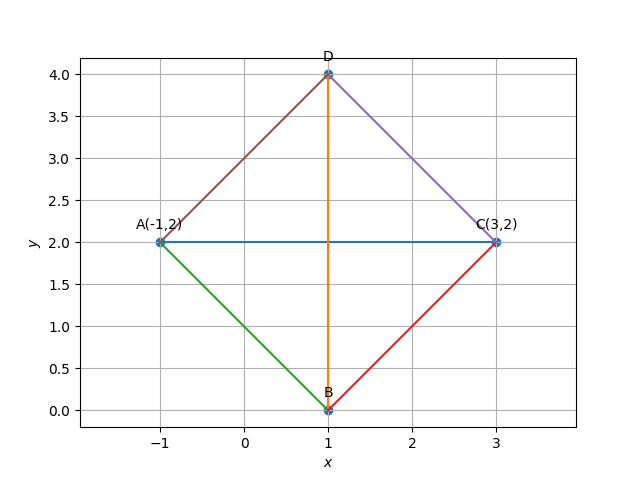
\includegraphics[width=\columnwidth]{chapters/10/7/4/4/figs/square}
	\end{center}
\caption{}
\label{fig:7/4/4/4Fig1}
\end{figure}

Shifting $\vec{A}$ to origin with reference to Fig. \ref{fig:7/4/4/4Fig2},
\begin{align}
\vec{A^{\prime}} =
\myvec{
0 \\
0\\
},
\vec{C^{\prime}} = \vec{C}-\vec{A} = 
\myvec{
4 \\
0\\
}
\end{align}

\begin{figure}[!h]
	\begin{center} 
	    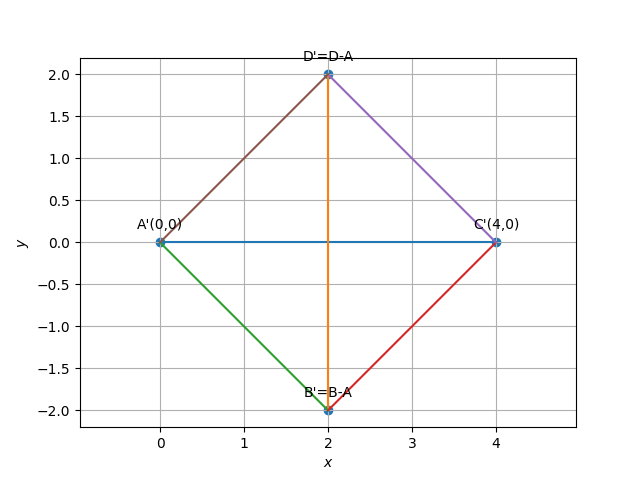
\includegraphics[width=\columnwidth]{chapters/10/7/4/4/figs/square1}
	\end{center}
\caption{}
\label{fig:7/4/4/4Fig2}
\end{figure}
\iffalse
In general,
the angle made by $AC$ with the x-axis is 
		\begin{align}
\beta = \theta + 45\degree
		\end{align}
\fi
Since
\begin{align}
\vec{C} - \vec{A} = \myvec{
4\\
0
} \equiv 
\myvec{
1\\
0
},
	\tan\theta&= \frac{0}{4} \implies 
\theta= 0\degree
\end{align}
		where
$\theta$ is the angle made by $AC$ with the x-axis.
Considering the rotation matrix 
\begin{align}
\vec{P} =
\myvec{
\cos\brak{\frac{\pi}{4}-\theta} & -\sin\brak{\frac{\pi}{4}-\theta} \\
\sin\brak{\frac{\pi}{4}-\theta} & \cos\brak{\frac{\pi}{4}-\theta} 
}
\end{align}
\iffalse
from Fig. \ref{fig:7/4/4/4Fig3},
\begin{align}
\vec{C^{\prime \prime}} = \vec{P}^\top (\vec{C}-\vec{A}) =
\myvec{
\frac{1}{\sqrt{2}} & -\frac{1}{\sqrt{2}} \\
\frac{1}{\sqrt{2}} & \frac{1}{\sqrt{2}}\\
}
\myvec{
4 \\
0\\
} = 
\myvec{
\frac{4}{\sqrt{2}} \\
\frac{4}{\sqrt{2}}\\
}
\end{align}
\begin{align}
\vec{B^{\prime \prime}} = \myvec{
 1&0\\
 0&0\\
}\vec{C^{\prime \prime}}=
\myvec{
 \frac{4}{\sqrt{2}}\\
 0\\
},
\vec{D^{\prime \prime}} = \myvec{
 0&0\\
 0&1\\
}\vec{C^{\prime \prime}}=
\myvec{
 0\\
 \frac{4}{\sqrt{2}}\\
} \text{ and }
\vec{A^{\prime \prime}} =
\myvec{
0 \\
0\\
}
\end{align}
\fi
\begin{figure}[!h]
	\begin{center} 
	    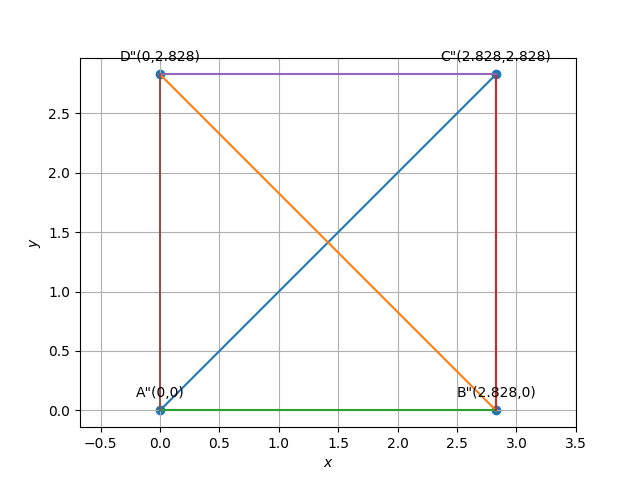
\includegraphics[width=\columnwidth]{chapters/10/7/4/4/figs/square2}
	\end{center}
\caption{}
\label{fig:7/4/4/4Fig3}
\end{figure}

\newpage
\iffalse
Again tranforming(rotating) the coordinates back to the original axis.

We know for anti-clockwise direction the rotation matrix is given as
\begin{align}
\vec{P} =
\myvec{
\cos\theta & -\sin\theta \\
\sin\theta & \cos\theta \\
}
\end{align}

Again we know that the angle is negative so the rotation will be in clockwise direction. So now the transformed(rotated) coordinates $\vec{B} \text{ and } \vec{D}$ are with refrence to 
\fi
from Figure 
%\ref{fig:7/4/4/4Fig4},
\ref{fig:7/4/4/4Fig3},
\begin{align}
	\vec{C^{\prime \prime}} &= \vec{P} (\vec{C}-\vec{A}) 
	\\
\label{eq:7/4/4/4bp}
	\vec{B^{\prime \prime}} &= \myvec{\vec{e}_1 & \vec{0}}\vec{C^{\prime \prime}}
	\\
\label{eq:7/4/4/4dp}
	\vec{D^{\prime \prime}} &= \myvec{ \vec{0} & \vec{e}_2}\vec{C^{\prime \prime}}
\end{align}
Now, 
\begin{align}
\label{eq:7/4/4/4b}
	\vec{B} = \vec{P}^{\top}\vec{B}^{\prime \prime}+\vec{A}
	\\
\label{eq:7/4/4/4d}
	\vec{D} = \vec{P}^{\top}\vec{D}^{\prime \prime}+\vec{A}
\end{align}
by reversing the process of translation and rotation.  Thus, 
from
\eqref{eq:7/4/4/4b}
\eqref{eq:7/4/4/4bp},
\eqref{eq:7/4/4/4d}
and
\eqref{eq:7/4/4/4dp}
\begin{align}
	\vec{B} = \vec{P}^{\top}\myvec{\vec{e}_1 & \vec{0}}\vec{P} (\vec{C}-\vec{A}) +\vec{A}
	\\
	\vec{D} = \vec{P}^{\top}\myvec{\vec{0} & \vec{e}_2  }\vec{P} (\vec{C}-\vec{A}) +\vec{A}
%	\vec{B} &= \brak{(\vec{C}-\vec{A})^{\top}\vec{P}^{\top} \vec{e}_1}\vec{P}^{\top}\vec{e}_1+\vec{A}
%	\\
%	\vec{D} &= \brak{(\vec{C}-\vec{A})^{\top}\vec{P}^{\top} \vec{e}_2}\vec{P}^{\top}\vec{e}_2+\vec{A}
\end{align}
yielding
		\begin{align}
\vec{B}=
\myvec{
1\\
0
},
\vec{D}
\myvec{
1\\
4
}.
		\end{align}
\iffalse
\begin{align}
\vec{B^{\prime}} &= \vec{P}\vec{B^{\prime \prime}} = \myvec{
\frac{1}{\sqrt{2}} & \frac{1}{\sqrt{2}} \\
-\frac{1}{\sqrt{2}} & \frac{1}{\sqrt{2}}\\
}
\myvec{
 \frac{4}{\sqrt{2}}\\
 0\\
} = 
\myvec{
2 \\
-2\\
}\\
\vec{D^{\prime}} &= \vec{P}\vec{D^{\prime \prime}} = \myvec{
\frac{1}{\sqrt{2}} & \frac{1}{\sqrt{2}} \\
-\frac{1}{\sqrt{2}} & \frac{1}{\sqrt{2}}\\
}
\myvec{
 0\\
 \frac{4}{\sqrt{2}}\\
} = 
\myvec{
2 \\
2 \\
}
\end{align}

\begin{figure}[!h]
	\begin{center} 
	    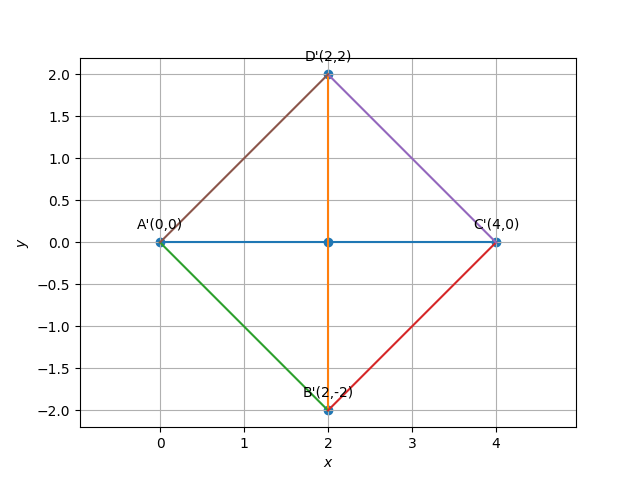
\includegraphics[width=\columnwidth]{chapters/10/7/4/4/figs/square3}
	\end{center}
\caption{}
\label{fig:7/4/4/4Fig4}
\end{figure}

Again transforming(shifting) the axis back to the original with refrence to Figure \ref{fig:7/4/4/4Fig5}
\begin{align}
\vec{B} &= \vec{B^{\prime}}+\vec{A} = \myvec{
2 \\
-2\\
}+\myvec{
-1 \\
2\\
} = 
\myvec{
1 \\
0\\
}\\
\vec{D} &= \vec{D^{\prime}}+\vec{A} = \myvec{
2 \\
2\\
}+\myvec{
-1 \\
2\\
} = 
\myvec{
1 \\
4 \\
}
\end{align}

Hence, the other two vertices are $\vec{B}(1,0) \text{ and } \vec{D}(1,4)$   

\begin{figure}[!h]
	\begin{center} 
	    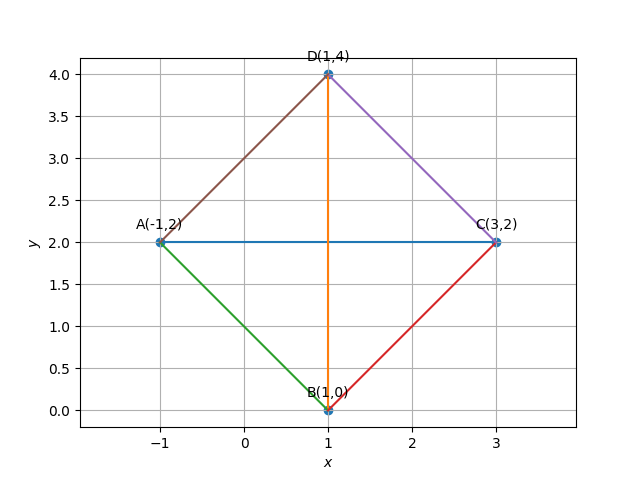
\includegraphics[width=\columnwidth]{chapters/10/7/4/4/figs/square4}
	\end{center}
\caption{}
\label{fig:7/4/4/4Fig5}
\end{figure}
which can also be expressed as
\begin{align}
\vec{B} &= \vec{A} + \vec{P}\myvec{
\vec{e_{1}}&\vec{0}\\
}
\vec{P}^\top \brak{\vec{C}-\vec{A}}\\
\vec{D} &= \vec{A} + \vec{P}\myvec{
\vec{0}&\vec{e_{2}}\\
}
\vec{P}^\top \brak{\vec{C}-\vec{A}}\\
\end{align}
where $\vec{P}$ is the rotation matrix and $\vec{A} \text{ and } \vec{C}$ are the position vectors of opposite vertices.

Derivation of the above formulas:

We know that after shifting the axis and rotating by the required angle any arbitrary square will be aligned with the x and y axis so that we can directly get the vectors $\vec{B} \text{ and } \vec{D}$ as follows
\begin{align}
\vec{C^{\prime\prime}} &= \vec{P}^\top \brak{\vec{C} - \vec{A}}\\
\vec{B^{\prime\prime}} &= \myvec{
\vec{e_{1}} & \vec{0}
}\vec{C^{\prime\prime}} = \myvec{
\vec{e_{1}} & \vec{0}
}\vec{P}^\top \brak{\vec{C} - \vec{A}}\\
\vec{B^{\prime}} &= \vec{P} \vec{B^{\prime\prime}}  = \vec{P}\myvec{
\vec{e_{1}} & \vec{0}
}\vec{P}^\top \brak{\vec{C} - \vec{A}}\\
\vec{B} &= \vec{A}+\vec{B^{\prime}}\\
 &= \vec{A} + \vec{P}\myvec{
\vec{e_{1}}&\vec{0}\\
}
\vec{P}^\top\brak{\vec{C}-\vec{A}}
\end{align}

Similarly for D it can be derived as
\begin{align}
\vec{C^{\prime\prime}} &= \vec{P}^\top \brak{\vec{C} - \vec{A}}\\
\vec{D^{\prime\prime}} &= \myvec{
\vec{0} & \vec{e_{2}}
}\vec{C^{\prime\prime}} = \myvec{
\vec{0} & \vec{e_{2}}
}\vec{P}^\top \brak{\vec{C} - \vec{A}}\\
\vec{D^{\prime}} &= \vec{P} \vec{D^{\prime\prime}} = \vec{P} \myvec{
\vec{0} & \vec{e_{2}}
}\vec{P}^\top \brak{\vec{C} - \vec{A}}\\
\vec{D} &= \vec{A}+\vec{D^{\prime}}\\
 &= \vec{A} + \vec{P}\myvec{
\vec{0}&\vec{e_{2}}\\
}
\vec{P}^\top\brak{\vec{C}-\vec{A}}
\end{align}


Verification of the above formula for the given question

\begin{align}
\vec{B} &= \myvec{
-1\\
2\\
}+\myvec{
\frac{1}{\sqrt{2}} & \frac{1}{\sqrt{2}} \\
-\frac{1}{\sqrt{2}} & \frac{1}{\sqrt{2}}\\
}\myvec{
 1&0\\
 0&0\\
}\myvec{
\frac{1}{\sqrt{2}} & -\frac{1}{\sqrt{2}} \\
\frac{1}{\sqrt{2}} & \frac{1}{\sqrt{2}}\\
}\myvec{
4\\
0\\
}\\
 &= \myvec{
-1\\
2\\
}+\myvec{
\frac{1}{\sqrt{2}} & \frac{1}{\sqrt{2}} \\
-\frac{1}{\sqrt{2}} & \frac{1}{\sqrt{2}}\\
}\myvec{
 1&0\\
 0&0\\
}\myvec{
\frac{4}{\sqrt{2}}\\
\frac{4}{\sqrt{2}}\\
}\\
 &= \myvec{
-1\\
2\\
}+\myvec{
\frac{1}{\sqrt{2}} & \frac{1}{\sqrt{2}} \\
-\frac{1}{\sqrt{2}} & \frac{1}{\sqrt{2}}\\
}\myvec{
\frac{4}{\sqrt{2}}\\
0\\
}\\
 &= \myvec{
-1\\
2\\
}+\myvec{
2\\
-2\\
}\\
 &= \myvec{
1\\
0\\
}\\
\vec{D} &= \myvec{
-1\\
2\\
}+\myvec{
\frac{1}{\sqrt{2}} & \frac{1}{\sqrt{2}} \\
-\frac{1}{\sqrt{2}} & \frac{1}{\sqrt{2}}\\
}\myvec{
 0&0\\
 0&1\\
}\myvec{
\frac{1}{\sqrt{2}} & -\frac{1}{\sqrt{2}} \\
\frac{1}{\sqrt{2}} & \frac{1}{\sqrt{2}}\\
}\myvec{
4\\
0\\
}\\
 &= \myvec{
-1\\
2\\
}+\myvec{
\frac{1}{\sqrt{2}} & \frac{1}{\sqrt{2}} \\
-\frac{1}{\sqrt{2}} & \frac{1}{\sqrt{2}}\\
}\myvec{
 0&0\\
 0&1\\
}\myvec{
\frac{4}{\sqrt{2}}\\
\frac{4}{\sqrt{2}}\\
}\\
 &= \myvec{
-1\\
2\\
}+\myvec{
\frac{1}{\sqrt{2}} & \frac{1}{\sqrt{2}} \\
-\frac{1}{\sqrt{2}} & \frac{1}{\sqrt{2}}\\
}\myvec{
0\\
\frac{4}{\sqrt{2}}\\
}\\
 &= \myvec{
-1\\
2\\
}+\myvec{
2\\
2\\
}\\
 &= \myvec{
1\\
4\\
}
\end{align}
\fi








\item The base of an equilateral triangle with side $2a$ lies along the y-axis such that the mid-point of the base is at the origin. Find vertices of the triangle.
\label{chapters/11/10/1/2}
\iffalse
\documentclass[journal,12pt,twocolumn]{IEEEtran}
\usepackage{graphicx}
\usepackage{listings}
\usepackage[utf8]{inputenc}
\usepackage{caption}
\usepackage{hyperref}
\usepackage[cmex10]{amsmath}
\usepackage{array}
\usepackage{gensymb}
\usepackage{booktabs}
\usepackage{etoolbox}
\patchcmd{\section}{\centering}{}{}{}
\providecommand{\norm}[1]{\left\lVert#1\right\rVert}
\providecommand{\abs}[1]{\left\vert#1\right\vert}
\let\vec\mathbf
\newcommand{\myvec}[1]{\ensuremath{\begin{pmatrix}#1\end{pmatrix}}}
\newcommand{\mydet}[1]{\ensuremath{\begin{vmatrix}#1\end{vmatrix}}}
\providecommand{\brak}[1]{\ensuremath{\left(#1\right)}}
\makeatletter
\newcommand\xleftrightarrow[2][]{%
  \ext@arrow 9999{\longleftrightarrowfill@}{#1}{#2}}
\newcommand\longleftrightarrowfill@{%
  \arrowfill@\leftarrow\relbar\rightarrow}
\makeatother
\title{Matrix Problems \textbf{\\Straight Lines }}
\author{Manoj Chavva} 

\begin{document}
\maketitle



\section{Problem Statement}

\noindent 
\fi
	\begin{figure}[!ht]
		\centering
 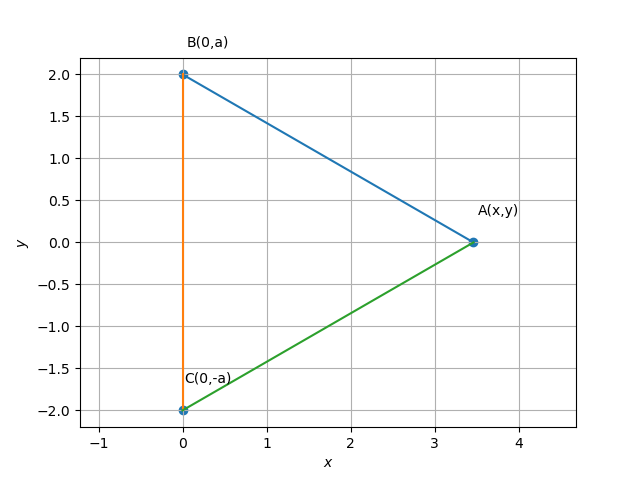
\includegraphics[width=\columnwidth]{chapters/11/10/1/2/figs/triangle.png}
		\caption{}
		\label{fig:11/10/1/2}
  	\end{figure}
	\\
	\solution Let the base be $BC$.  From the given information, 
\begin{align}
	\vec{B} = a\vec{e}_2,
	\vec{C} = -a\vec{e}_2
\end{align}
Since $\vec{A}$ lies on the $x$-axis, 
\begin{align}
	\vec{A} = k\vec{e}_1
\end{align}
and 
\begin{align}
	\norm{\vec{A}-\vec{C}}^2 &= \brak{2a}^2
	\\
	\implies \norm{\vec{A}}^2+\norm{\vec{C}}^2 - 2 \vec{A}^{\top}\vec{C} &= 4a^2
	\\
	\implies k^2 +a^2 &= 4a^2
	\\
	\text{or, } k = \pm a\sqrt{3}
\end{align}
Thus, 
\begin{align}
	\vec{A} = \pm \sqrt{3}a\vec{e}_1
\end{align}
		Fig. \ref{fig:11/10/1/2}
		is plotted for $a = 2$.

\iffalse

\begin{figure}[h]
\includegraphics[width=1\columnwidth]{triangle.png}
\caption{Equilateral Triangle ABC}
\label{fig:triangle}
\end{figure}

\section{Construction}
B and C are the inputs.
\begin{table}[h]
\centering
\large
\begin{tabular}{|l|l|l|}
\hline
\textbf{Symbol} & \textbf{Value} & \textbf{Description} \\ \hline
B               & \myvec{0 \\ 2}         & Vertex B             \\ \hline
C               & \myvec{0 \\ -2}        & Vertex C             \\ \hline
A               & \myvec{x \\ y}          & Vertex A             \\ \hline
A1              & \myvec{x1 \\ y1}       & Vertex A             \\ \hline
\end{tabular}
\end{table}

\section{Solution}
\noindent Given the base with 2a is lies on the y-axis with the mid-point of the base is at origin. The vertices of the two points on y-axis will be

\begin{equation}
\vec{B}=\begin{pmatrix} 
0\\
a
\end{pmatrix}, {
\vec{C}=\begin{pmatrix} 
0\\
-a
\end{pmatrix} }
\end{equation}
\noindent Given $\Delta$ABC is an equilateral triangle i.e 
\begin{equation}
 \norm{\vec{A}-\vec{B}}= \norm{\vec{B}-\vec{C}}= \norm{\vec{C}-\vec{A}} =2a
\end{equation}

%\noindent As AB = AC, triangle is isoceles and by properties of isoceles triangle, altitude is perpendicular bisector of base.\\
%
%\noindent Therefore $\angle$AOC = $\angle$AOB = $90^0$ and $\norm{\vec{O}-\vec{B}}= \norm{\vec{O}-\vec{C}}= a$ \\
%
%\noindent By Cosine laws,
%\begin{equation}
%\cos\vec{B} = \cos\vec{C} = a* \frac{1}{2a} = \frac{1}{2}
%\end{equation}
%\begin{equation}
%\angle B = \angle C = \arccos\frac{1}{2} = 60^0
%\end{equation}
% \begin{equation}
% \angle A = 180^0 -(60^0 * 2) = 60^0
%  \end{equation}
%\noindent Therefore, the equilaterial triangle have all internal angles eaqual to  $60^0$ 

\noindent Consider, two sides of equilateral triangle be $\vec{A}$ and $\vec{B}$ then the third side will be $ \vec{A} -\vec{B}$ 
%Hence,
%\begin{equation}
%\norm{\vec{a}-\vec{b}}^2 = l
%\end{equation}
%\begin{equation}
%\brak{\vec{a}-\vec{b}}^{\top} \brak{\vec{a}-\vec{b}} = l^2
%\end{equation}
%\begin{equation}
%l^2 = 2 \vec{a}^{\top} \cdot \vec{b}
%\end{equation}
%\begin{equation}
%l^2 = 2 \norm{\vec{a}}\norm{\vec{b}} \cos\theta
%\end{equation}
%\begin{equation}
%\theta = \arccos\frac{1}{2} = 60^0
\begin{equation}
\norm{\vec{A}}=\norm{\vec{B}}=\norm{\vec{A-B}}\\
\end{equation}
\begin{equation}
\norm{\vec{A}}^2=\norm{\vec{B}}^2=\norm{\vec{A-B}}^2\\
\end{equation}
\begin{equation}
\norm{\vec{A}}^2+\norm{\vec{B}}^2-2\vec{A}^T\vec{B}=\norm{\vec{A}}^2=\norm{\vec{B}}^2\\
\end{equation}
\begin{equation}
\frac{\vec{A}^T\vec{B}}{\norm{\vec{A}}^2}=\frac{\vec{A}^T\vec{B}}{\norm{\vec{B}^2}}=\frac{1}{2}
\end{equation}
%$\triangle$OAB is a equilateral triangle\\

\noindent Therefore, the  triangle have all internal angles eaqual to  $60^0$

The angle between two vectors is given by 
  \begin{align}
    \label{eq:angle2d}
    \theta = \cos^{-1}\frac{\vec{A}^{\top} \vec{B}}{\norm{A}\norm{B}}
  \end{align}

 \begin{equation}  
  \brak{\vec{x}-\vec{B}}^{\top} \brak{\vec{x}-\vec{C}}= \norm{\vec{x}-\vec{B}} \cdot \norm{\vec{x}-\vec{C}} \cdot \cos\theta 
 \end{equation}

 \begin{equation}  
\brak{\vec{x}^\top \cdot \vec{x}} - \brak{\vec{x}^\top \cdot \vec{C}} - \brak{\vec{B}^\top \cdot \vec{x}} - \brak{\vec{B}^\top \cdot \vec{C}} = 2a \cdot 2a \cos 60^0   
 \end{equation}

 \begin{equation}  
\norm{\vec{x}}^2 - \vec{x}^\top\brak{\vec{B}+\vec{C}} - \vec{B}^\top \cdot \vec{C} = 2a \cdot 2a \cdot \frac{1}{2}
 \end{equation}

  \begin{equation}  
\norm{\vec{x}}^2 - \vec{x}^\top\brak{0} -\myvec{0 \\ a} \myvec{0 & -a}  = 4a^2
 \end{equation}

\begin{equation}
\norm{\vec{x}}^2 + a^2 = 4a^2
\end{equation}

\begin{equation}
\norm{\vec{x}}^2 = 3a^2
\label{eq-1}
\end{equation}
Considering, the line equation of $\vec{AB}$

\begin{equation}
\norm{\vec{x}-\vec{B}}^2 = 4a^2
\end{equation}

\begin{equation}
\brak{\vec{x} -\vec{B}}^{\top} \cdot \brak{\vec{x}-\vec{B}} = 4a^2
\end{equation}

\begin{equation}
\norm{\vec{x}}^2-2\cdot \vec{x}^\top \vec{B} + \norm{\vec{B}}^2 = 4a^2
\end{equation}

\begin{equation}
3a^2 - 2\cdot \vec{x}^\top \vec{B} + a^2 = 4a^2
\end{equation}

\begin{equation}
\vec{x}^\top \vec{B} = 0
\end{equation}
\noindent Since we can write, \begin{equation}
\vec{B} = a \cdot \vec{e}_2
\end{equation}

\begin{equation}
\vec{x}^\top \cdot a \cdot \vec{e}_2 = 0
\end{equation}

\begin{equation}
\vec{x}^\top \cdot \vec{e}_2 = 0
\end{equation}

\begin{equation}
\vec{x} = \lambda \vec{e}_1
\end{equation}

\noindent From this its clearly concluded that third vertex will lie on x-axis. 
\noindent From the equation \eqref{eq-1} 
\begin{equation}
\vec{x} = \sqrt{3}{a}
\end{equation}


\noindent Hence,the coordinates of the vertices of triangle are 
  \begin{equation*}
\vec{A} = 
   \begin{pmatrix}
   \pm\sqrt{3}a \\ 0
 \end{pmatrix}
 \end{equation*}

\begin{equation}
\vec{B}=\begin{pmatrix} 
0\\
a
\end{pmatrix}, {
\vec{C}=\begin{pmatrix} 
0\\
-a
\end{pmatrix} }
\end{equation}



\begin{table}[h]
\large
\begin{tabular}{lll}
\multicolumn{3}{l}{Get Python Code for image from}                                                 \\ \hline
\multicolumn{3}{|l|}{\url{https://github.com/ManojChavva/FWC/blob/main/Matrix/line/code-py/triangle.py}} \\ 
 \hline
\multicolumn{3}{l}{Get LaTex code from}                                                            \\ \hline
\multicolumn{3}{|l|}{\url{https://github.com/ManojChavva/FWC/blob/main/Matrix/line/line.tex}}            \\ \hline
\end{tabular}
\end{table}

\end{document}

\fi

\item Without using distance formula, show that points (– 2, – 1), (4, 0), (3, 3) and (–3, 2) are the vertices of a parallelogram.
\label{chapters/11/10/1/9}
	  From \eqref{eq:two-pgm},
\begin{align}
\vec{A}-\vec{B} = 
\vec{D}-\vec{C} =  \myvec{-6\\-1}
\end{align}
Hence, $ABCD$ is a parallelogram.
See \figref{fig:chapters/11/10/1/91}.
\begin{figure}[h!]
  \centering
   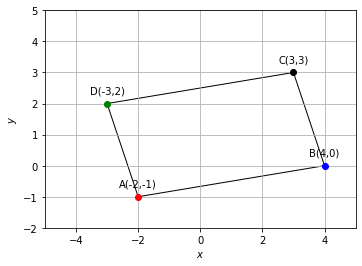
\includegraphics[width=\columnwidth]{chapters/11/10/1/9/figs/paralellogram.png}
    \caption{}
     \label{fig:chapters/11/10/1/91}  
\end{figure}




\item A line passes through $(x_1,y_1)$ and $(h,k)$. If slope of the line is m show that $(k-y_1)=m(h-x_1)$.
\label{chapters/11/10/1/12}
The direction vector
\begin{align}
	\vec{B}-\vec{A}
	=
	\myvec{
  h-x_1\\
  k-y_1
  }
   \equiv
	\myvec{
1\\
	\frac{ k-y_1}{h-x_1}
  }
  \\
	\implies m = 
	\frac{ k-y_1}{h-x_1},
\end{align}
yielding the desired result.

\item Consider the following population and year graph, Find the slope of the line AB and using it, find what will be the population in the year 2010?
\\
\begin{figure}[!ht]
\centering
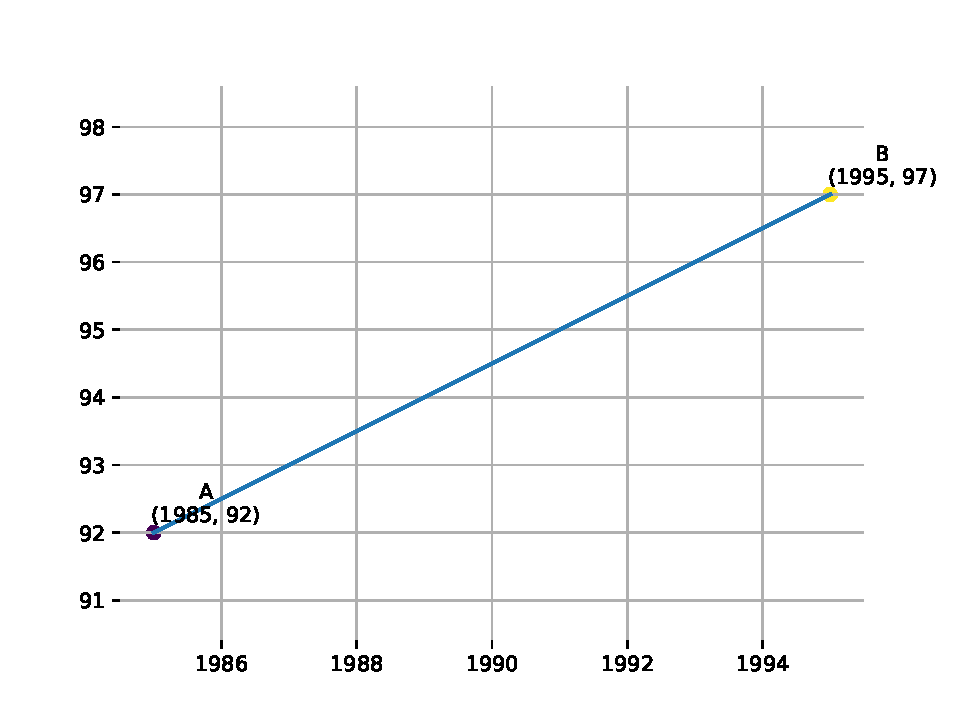
\includegraphics[width = \columnwidth]{chapters/11/10/1/14/figs/fig.png}
\caption{}
\label{fig:chapters/11/10/1/14/1}
\end{figure}
\solution
The direction vector of the line in \figref{fig:chapters/11/10/1/14/1} is
\begin{align}
\vec{m} = \vec{B} - \vec{A}
= \myvec{2 \\ 1}
\\
\implies \vec{n}
= \myvec{1 \\ -2}
\end{align}
 The equation of the line is then given by 
\begin{align}
\vec{n}^{\top} (\vec{x} -\vec{A}) &= 0 \\
\implies 
\myvec{1& -2} \vec{x} &= 1801
\\
\implies  \myvec{1&-2} \myvec{2010\\y} &= 1801 \\
\implies y &= \frac{209}{2}
\end{align}





\item Find a vector of magnitude 5 units, and parallel to the resultant of the vectors $\vec{a}=2\hat{i}+3\hat{j}-\hat{k}$ and $\vec{b}=\hat{i}-2\hat{j}+\hat{k}$.\\

\item Let $\vec{a}$ and $\vec{b}$ be two unit vectors and $\theta$ is the angle between them. Then $\vec{a}+\vec{b}$ is a unit vector if
	\begin{enumerate}
		\item $\theta = \frac{\pi}{4}$
		\item $\theta = \frac{\pi}{3}$
		\item $\theta = \frac{\pi}{2}$
		\item $\theta = \frac{2\pi}{3}$
			\end{enumerate}
\solution
Given,
\begin{align}
	\norm{\vec{a}}=\norm{\vec{b}}=1\label{eq:12/10/5/17/1}
	\\
	\norm{\vec{a}+\vec{b}}=1\label{eq:12/10/5/17/2}
\end{align}
Squaring both sides of \eqref{eq:12/10/5/17/2}  , we get
\begin{align}
	\norm{\vec{a}+\vec{b}}^2=1^2
\\	
	\implies \norm{\vec{a}}^2 + \norm{\vec{b}}^2 + 2\vec{a}^{\top}\vec{b} = 1\label{eq:12/10/5/17/3}	
\end{align}
Substituting \eqref{eq:12/10/5/17/1} in \eqref{eq:12/10/5/17/3}, we get
\\
\begin{align}
	\implies 1+1+2(\norm{\vec{a}}\norm{\vec{b}}\cos{\theta})=1
	\\
	\implies 2+2(\norm{\vec{a}}\norm{\vec{b}}\cos{\theta})=1
        \\
	\implies 2(\norm{\vec{a}}\norm{\vec{b}}\cos{\theta})=-1
	\\
	\implies (\norm{\vec{a}}\norm{\vec{b}}\cos{\theta})=\frac{-1}{2}\label{eq:12/10/5/17/4}
\end{align}
Subtituting \eqref{eq:12/10/5/17/1} in \eqref{eq:12/10/5/17/4}, we get
\begin{align}
	\implies \cos{\theta}=\frac{-1}{2}
	\\
	\implies \theta=\frac{2\pi}{3}
\end{align}

\\
\begin{figure}[!ht]
	\centering
	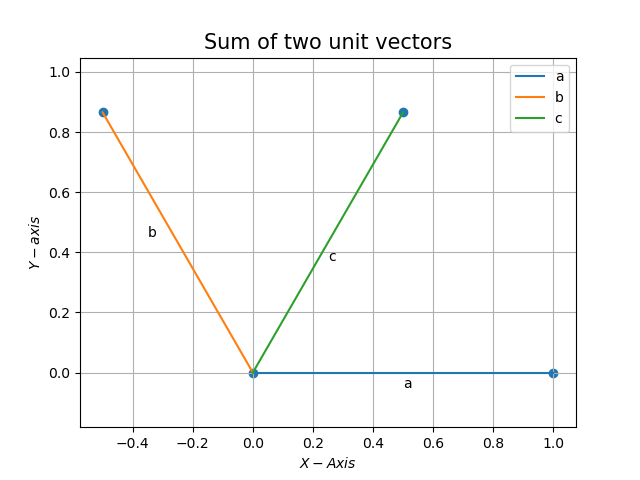
\includegraphics[width=\columnwidth]{chapters/12/10/5/17/codes/Python/figs/fig.png}
	\caption{$\vec{OA}$ and $\vec{CO}$ is $\vec{a}$ and $\vec{OB}$ is $\vec{b}$ and $\vec{CB}$ is $\vec{a+b}$}
	\label{fig:12/10/5/17}
\end{figure}
	\item $\vec{AB}$ is a line segment and $\vec{P}$ is its mid-point. $\vec{D}$ and $\vec{E}$ are points on the same side of $\vec{AB}$ such that $\angle BAD = \angle ABE$ and $\angle EPA = \angle DPB$. Show that
		\begin{enumerate}
			\item $\triangle \vec{DAP} \cong  \triangle \vec{EBP}$
			\item $\vec{AD} = \vec{BE}$
\end{enumerate}
\begin{figure}[!ht]
	\centering
    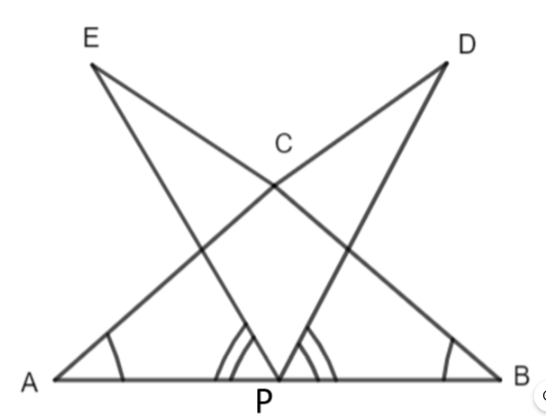
\includegraphics[width=\columnwidth]{figs/mc.png}
	\caption{$\triangle  \vec{DAP} \hspace{12pt} and \hspace{12pt} \triangle \vec{EBP}$}
 \label{fig:fig1}
\end{figure}
\textbf{Construction steps:}
		\begin{enumerate}[label=(\roman*)]
\item Let assume, the input parameters are, 
\begin{table}[!ht]
\centering
	\begin{tabular}{|c|c|p{5cm}|}
\hline
\textbf{Parameter} & \textbf{Value} & \textbf{Description} \\
\hline
$\theta_1$ & $30\degree$ & $\angle{BAD} = \angle{ABE}$ \\
\hline
$\theta_2$ & $60\degree$ & $\angle{EPA} = \angle{DPB}$ \\
\hline
	$\vec{A}$ & $\myvec{0\\0}$ & Reference point at origin \\
\hline
	$\vec{B}$ & $\myvec{5\\0}$ & point $\vec{B}$ on the same axis of $\vec{A}$ \\
\hline

\end{tabular}

	  \caption{Input Parameters}
	  \label{Table-1: }
\end{table}
$\therefore$ the output can be calculated as,
\begin{table}[!ht]
\centering
	\begin{tabular}{|c|c|p{5cm}|}
\hline
\textbf{Parameter} & \textbf{Value} & \textbf{Description} \\
\hline
	$r$ & $\norm{A-B}$ & Length of $\vec{AB}$ \\
\hline
	$\vec{P}$ & $\frac{\vec{A+B}}{2}$ & Mid-point of $\vec{AB}$ \\
\hline
	$\vec{D}$ & $\vec{A}$ + $\myvec{r \cos \theta_1  \\ r \sin \theta_1}$ & From point $\vec{A}$ makes an angle $\theta_1$ in anticlock-wise with line $\vec{(AB, AD)}$  \\
\hline
	$\vec{E}$ & $\vec{B}$ + $\myvec{-r \cos \theta_1  \\ r \sin \theta_1}$ & From point $\vec{B}$ makes an angle $\theta_1$ in clock-wise with line $\vec{(AB, BE)}$  \\  
\hline       
	$\vec{D}$ & $\vec{P}$ + $\myvec{r \cos \theta_2  \\ r \sin \theta_2}$ & From point $\vec{P}$ makes an angle $\theta_2$ in anticlock-wise with line $\vec{(BP, DP)}$  \\  
\hline
	$\vec{E}$ & $\vec{P}$ + $\myvec{-r \cos \theta_2  \\ r \sin \theta_2}$ & From point $\vec{P}$ makes an angle $\theta_2$ in anticlock-wise with line $\vec{(AP, EP)}$  \\  
\hline
\end{tabular}

	  \caption{Output Parameters}
	  \label{Table-2: }
\end{table}
$\therefore$ By, joining these points forms the required figure
\begin{figure}[!ht]
	\centering
    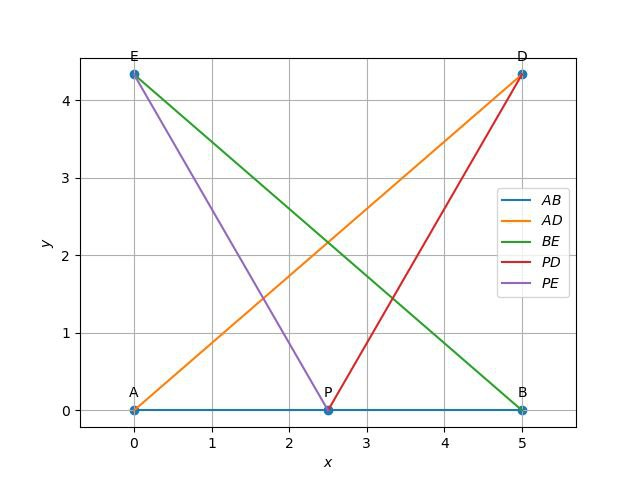
\includegraphics[width=0.8\columnwidth]{figs/fig_math_comp}
	\caption{$\triangle \vec{DAP} \hspace{12pt} and \hspace{12pt} \triangle \vec{EBP}$}
    \label{fig:fig2}
\end{figure}
\end{enumerate}
\end{enumerate}
